\documentclass[10pt,a4paper]{article}
\usepackage[margin=2.2cm]{geometry}
\usepackage{amsmath,amssymb}
\usepackage{graphicx}
\usepackage{booktabs}
\usepackage{tabularx}
\usepackage{xcolor}
\usepackage{enumitem}
\usepackage[hidelinks]{hyperref}
\usepackage{titlesec}
\usepackage{parskip}
\setlist{nosep,leftmargin=1.4em}
\titleformat{\section}{\large\bfseries}{\thesection}{0.6em}{}
\titleformat{\subsection}{\normalsize\bfseries}{\thesubsection}{0.6em}{}
\newcommand{\eav}{\varepsilon_{Av}}
\newcommand{\eam}{\varepsilon_{Am}}
\newcommand{\cneed}[1]{\textcolor{red}{[CITE: #1]}}
\newcommand{\confirm}[1]{\textcolor{blue}{#1}}
\newcolumntype{L}{>{\raggedright\arraybackslash}X}

\begin{document}

\begin{center}
{\LARGE\bfseries Narrative outline}\\[4pt]
{\large Decoupling the Dyad: Private Partner Models in a Coupled-Oscillator Model of Attachment for Robot Dyads}\\[4pt]
Target: \emph{IEEE Transactions on Cognitive and Developmental Systems} (TCDS)\\
Draft prepared from the AttachmentNN repository; companion to \texttt{papers/tcds/draft/main.pdf}
\end{center}

\section{Positioning: three documents, three roles}

\begin{tabularx}{\textwidth}{@{}p{3.1cm}LL@{}}
\toprule
Document & What it contains & Role in the new paper \\
\midrule
Living Machines 2024 (LM, published, LNAI 14930) & Coupled-oscillator model; ambivalent/avoidant regimes; two physical MiRo robots with one central controller (code: \texttt{ros\_mommy\_daddy}). & \textbf{Cited support.} The model is restated in one short section and never re-derived; the physical-robot results are cited, not reproduced. \\
npj Robotics draft (rejected for similarity to LM) & LM plus extended analysis of the coupled model: saddle-node / route to chaos, relative-phase map, slowing before transitions, agent-based SSP simulation, real-robot heat maps and $\chi^2$. & \textbf{Supporting analysis / coupled baseline.} Its findings define what the \emph{coupled} model predicts; the new paper shows how \emph{decoupling} changes them. Unpublished, so it is referred to with a placeholder; posting it as a preprint would make it citable. \\
New TCDS paper (AttachmentNN) & Decoupled controllers with private partner models and learned coupling estimates, in six variants; 577 validated Gazebo runs; offline analyses from random starting needs. & \textbf{The contribution.} Everything in Sections IV--VIII of the draft is new. \\
\bottomrule
\end{tabularx}

The npj rejection came from overlap with LM. The new paper avoids it by (i) leading with a question LM could not ask (what happens when each agent must carry its own model of the other), (ii) keeping the model recap to one section with equations only, and (iii) building every result section on AttachmentNN data or analyses. An 8-gram overlap check of the draft against the LM PDF and the npj source finds 0.45\% and 0.74\% shared 8-grams, all in author names, affiliations, funding, the declaration of interest and one reference title.

\section{Title and thesis}

\textbf{Working title.} \emph{Decoupling the Dyad: Private Partner Models in a Coupled-Oscillator Model of Attachment for Robot Dyads.}

\textbf{One-sentence thesis.} Attachment-like phase relations in a coupled-oscillator dyad survive the move to private needs only when each agent's model of its partner is anchored to the partner: with private models and learned coupling alone the realised synchrony and anti-synchrony vanish while each agent keeps believing in them, and a partner model propagated with the standard model and driven by what the robot senses brings the ambivalent anti-synchrony back.

\section{What changed since the first draft, and why}
\begin{itemize}
\item \textbf{The avoidant synchrony of the decoupled controller was an artefact of the identical start.} Every earlier run started both agents from $(-1,1,-1,1)$. From random starting needs the decoupled avoidant dyad is uncorrelated (median $r\approx0$) and each agent's belief is anti-synchronised. The identical start is an invariant but unstable state: a difference of $10^{-7}$ grows until the needs separate after 704~s at $\eav=0.1$. The coupled controller is robust (r = 1.00 from any start). Section IV/V of the draft were rewritten around this.
\item \textbf{The estimation question was made explicit and tested.} Following your framing: the current agent's learned coupling is the \emph{estimator} of how the partner pulls on it; the partner model is the agent's estimate of the partner's state, either sharing the learned estimate (as in the original controller) or following the standard model as a baseline. New controller modes feed the networks what the robot senses (ground-truth or odometry distance, the calls on the audio topics), as in training.
\item \textbf{All Gazebo evidence was repeated and extended:} 577 runs (from 20), seeded random starts, both controllers, six variants, off-axis points and 900~s runs. Every run is validated against its controller (replay or logged-input check; 557/557 pass).
\end{itemize}

\section{The narrative arc}
\begin{enumerate}[leftmargin=1.6em]
\item \textbf{Problem.} The coupled model of LM reproduces secure/avoidant/ambivalent signatures, but one integrator holds both needs. In a real dyad needs are private; partners act on working models of each other \confirm{(Bowlby 1982 --- verify the passage)}.
\item \textbf{Decoupling.} Each robot integrates its own oscillator plus a partner model; its estimate of the coupling comes from networks trained on interaction signals in an agent-based SSP.
\item \textbf{What decoupling changes} (from random starts). Coupled: synchrony under avoidance, anti-synchrony under ambivalence. Decoupled: realised $r\approx0$ in both, beliefs anti-synchronised; the two private models detune (24.8 vs 31.5~mHz at $\eam=0.2$). Identical starts hide this (unstable symmetric state).
\item \textbf{Estimating the partner.} Child's learned estimate follows the true coupling when it hears the calls (0.84--0.97), inverted under avoidance when silent ($-0.51$); caregiver's estimate poor in all variants. A good estimate does not keep a partner model that shares it on the partner ($r\approx0.1$). A standard-model partner + sensing does: $r(\hat{x}_p,x_p)=0.60$--0.91 for $\eam=0.1$--0.4, ambivalent anti-synchrony restored ($r=-0.51$ to $-0.69$), at the cost of escaping at weaker coupling.
\item \textbf{Embodiment.} Robots express the regimes: call reciprocity is 1.00 (coupled, avoidance) vs $\approx$0.3 (coupled, ambivalence) vs wandering 0.2--1.0 (decoupled).
\item \textbf{Inference.} Observer of both robots: 89\% of 176 Gazebo runs (child only: 60\%).
\item \textbf{Outlook.} Explicit observer correcting the partner model (pulse coupling at calls); bounded coupling; physical robots; people; ethics.
\end{enumerate}

\section{Research questions and answers}
\begin{tabularx}{\textwidth}{@{}p{4.3cm}L@{}}
\toprule
RQ & Answer (numbers as in the draft) \\
\midrule
RQ1 What does decoupling change, from generic starts? & Coupled keeps $r=+1$ (avoidance) and $-1$ (ambivalence). Decoupled realised $r$ within 0.11 of 0 for $\varepsilon=0.1$--0.4; belief $-0.50/-0.81$ (avoidance), $-0.94$ to $-0.99$ (ambivalence). Identical start unstable: $10^{-7}\to$704/421~s, $10^{-3}\to$322/188~s, $0.1\to$17--18~s. Over the plane 94\% (coupled) and 89\% (decoupled) of starts escape. \\
RQ2 How well does each agent estimate the partner? & Child estimator 0.97 (avoidance) / 0.84 (ambivalence) with sensing; $-0.51$ under avoidance when silent; caregiver $-0.48$ to 0.27. Partner model tracks the partner only with standard-model propagation + sensing (0.60--0.91). \\
RQ3 Do robots express the regimes? & 557/557 runs validated. Reciprocity at $\varepsilon=0.2$: coupled 1.00 (Av) / 0.29 (Am); decoupled 0.60 / 0.65; standard-model partner + sensing 0.24--0.44 under ambivalence. \\
RQ4 Can behaviour reveal the parameters? & Child only 60\% (106/176); both robots 89\% (156/176), identical 88\% / random 89\%; Gazebo-only CV 56\% / 74\%. \\
\bottomrule
\end{tabularx}

\begin{figure}[h]
\centering
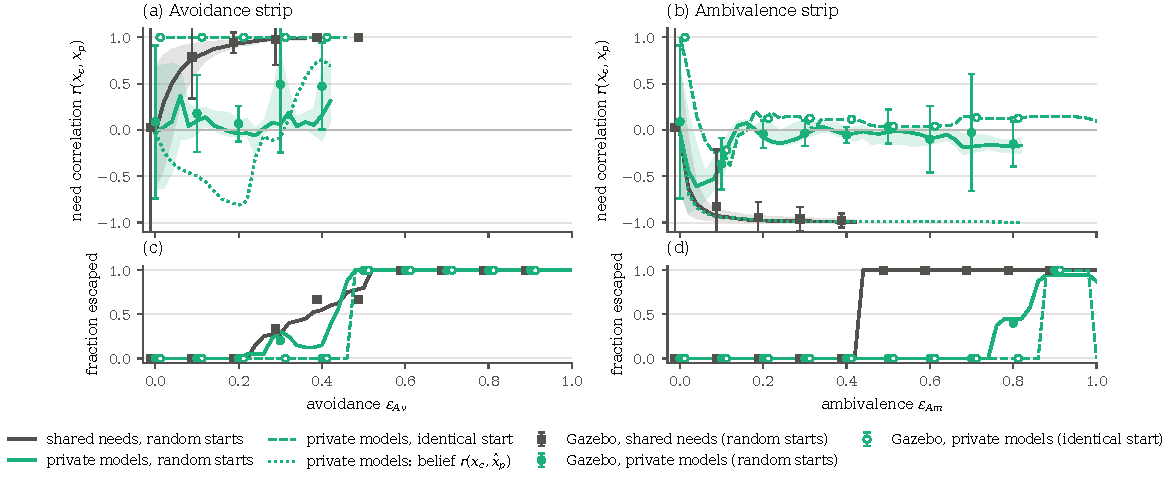
\includegraphics[width=\textwidth]{../draft/figures/fig_strips.pdf}
\caption{The central figure (draft Fig.~3): coupled vs decoupled from random starts, the identical-start artefact (dashed) and the Gazebo runs.}
\end{figure}

\section{Contributions as they should be stated}
\begin{enumerate}[leftmargin=1.6em]
\item A decoupled formulation with private partner models and learned coupling estimates, in variants that differ in what the estimator senses and how the partner model is propagated.
\item A dynamical comparison from random starting needs: the coupled dyad keeps its phase relations; the decoupled dyad loses its realised phase relation while beliefs persist; identical starts are an unstable artefact.
\item An estimation analysis: the learned estimate works when the child hears the partner; only a standard-model partner model anchored by sensing follows the partner and restores anti-synchrony.
\item 577 validated Gazebo runs, with call reciprocity as a behavioural signature.
\item Recovery of attachment parameters from behaviour (89\%), with the caregiver's behaviour carrying most information.
\end{enumerate}

\section{Section-by-section blueprint}
\begin{tabularx}{\textwidth}{@{}p{3.3cm}Lp{3.2cm}@{}}
\toprule
Section & Argument & Evidence \\
\midrule
I Introduction & Private needs; four questions; contributions; relation to LM & Table I; Fig.~1 \\
II Background & Dimensional attachment; models; coupled oscillators; estimating the partner & LM/npj refs + placeholders \\
III Controller & Equations; where $d_p,d_e$ come from; six variants & Eqs.~1--4; Tables II--III \\
IV Decoupling & Private partner model; estimator inputs; partner propagation; learned estimates & Eqs.~5--6; Fig.~2 \\
V What decoupling changes & Coupled robust; decoupled loses realised phase; identical start unstable; plane; escape & Figs.~3--5; App.~B \\
VI Estimating the partner & Offline accuracy; Gazebo estimator and partner-model tracking by variant & Fig.~6--7; Table IV \\
VII Gazebo & Setup; validation of all runs; behaviour and reciprocity; long runs; stand-in & Figs.~8--11; Table V \\
VIII Inverse problem & Child vs dyad observer & Fig.~12; Table VI \\
IX Discussion & Belief vs reality; what estimation needs; identical starts and validation; physical robots; limitations; HRI & --- \\
\bottomrule
\end{tabularx}

\section{Figures and tables}
All figures are generated by \texttt{analysis/tcds/figures.py}; Figs.~1--2 are TikZ diagrams in \texttt{draft/diagrams/}. New since the first draft: Fig.~7 (estimation by variant), Fig.~11 (900~s runs), the stability figure (appendix), Table IV (estimation), Table V (behaviour by condition). Redesigned from new data: Figs.~3, 4, 5, 8, 9, 12.

\section{Reference strategy}
\textbf{Allowed sources:} the union of the LM and npj reference lists (\texttt{refs.bib}, 37 entries). Anything else appears as a red \cneed{description} placeholder, never an invented reference; the draft lists them in an appendix. Current placeholders:
\begin{enumerate}[leftmargin=1.6em]
\item partner or user state estimation / theory of mind in social robotics
\item extended analysis of the coupled model (npj draft), if released as a preprint
\item internal/forward models of other agents in social cognition and robotics
\item learning coupling functions or interaction dynamics with neural networks
\item state estimation / observers for coupled oscillators
\item ROS and Gazebo
\item AprilTag fiducial detection
\item random forests
\item ethics of affect-adaptive social robots
\end{enumerate}
Worth adding once sourced: instability of synchronous manifolds / symmetry breaking in coupled oscillators; phase drift under frequency detuning; observers and Kalman-type filters for oscillator phase.

\textbf{Issues found in the existing reference lists (please check):}
\begin{itemize}
\item LM ref.~29, Paxton et al.\ 2011 (MESA), is a \emph{stellar astrophysics} code, not the Mesa agent-based modelling framework. It is excluded from \texttt{refs.bib} and must not be cited.
\item Craig: LM cites the 2002 \emph{Nature Reviews Neuroscience} article, npj the 2015 Princeton book. These are different works; \texttt{refs.bib} keeps the article.
\item Prescott et al.\ 2017 (MiRo, HRI): the DOI is printed as \texttt{10.1145/10.1145/...} in both lists (prefix doubled); corrected in \texttt{refs.bib}.
\item Year mismatches: Ca\~namero et al.\ (2006 vs 2011; the DOI suggests 2006), Palumbo et al.\ (2016 vs 2017), Ainsworth et al.\ (1978 original vs 2015 reprint), Wilson \& Prescott (key 2021, year 2022).
\item Atkinson et al.\ 2006, \emph{Mathematical Models of Mother/Child Attachment}: venue and publisher missing in LM.
\end{itemize}

\section{Items for the authors to confirm}
\begin{enumerate}[leftmargin=1.6em]
\item In the decoupled and baseline variants both robots load the caregiver's networks (as in the original controller); the sensing variants use each robot's own networks. Keep this split?
\item The child's audio detector listened to its own channel; fixed for all new runs (flagged \texttt{audio\_fix} in \texttt{meta.json}). It affected only tail wagging and the recorded evidence trace.
\item Training data: only $\varepsilon=0$ found a recorded run; the other values came from the agent simulator.
\item The training filter for the distance (\texttt{filter\_dist}) is a \texttt{conv1d}, which puts the largest weight on the oldest of the 20 samples. The sensing controllers reproduce it as trained; intended?
\item Escape at strong avoidance (and, from random starts, from $\eav\approx0.24$): report as a model property (current draft) or add a bounded variant?
\item Runs 17--33: which controller produced them? (not used)
\item Bowlby (1982) page; ROS, Gazebo and MDK versions; repository URL; funding text.
\item Whether to post the npj manuscript as a preprint so it can be cited.
\end{enumerate}

\section{Anticipated reviewer questions}
\begin{itemize}
\item \emph{``Is the learned coupling really estimating the partner?''} Section VI scores it against the coupling of both robots' true needs on every run, and separates the estimate from the partner model.
\item \emph{``Results depend on the initial condition.''} All main results are from random starting needs; the identical start is analysed as an unstable special case.
\item \emph{``Simulation only.''} The physical demonstration is LM; Gazebo adds ground truth, controller logs and 577 validated runs; odometry drift ($\approx$1~m per run) motivates ground truth.
\item \emph{``Few runs per condition.''} The needs are deterministic given the start (replay validated), so needs-level results rest on 40 offline starts per value; Gazebo adds behaviour with 3--5 seeds.
\item \emph{``How does this differ from LM?''} Table I, Section I-A and the cover letter.
\end{itemize}

\section{Cover-letter paragraph (draft)}
\begin{quote}
This manuscript extends our conference paper ``A coupled-oscillator model of human attachment dynamics evaluated in a robot dyadic interaction'' (Living Machines 2024, LNAI 14930, pp.~52--67). The conference paper introduced the model and demonstrated it on two physical robots controlled by a single integrator that held both agents' needs. The present manuscript asks what happens when the needs are private and each robot must estimate its partner. We restate the model's equations in one section and do not repeat the derivation or the physical-robot experiment. All analyses and results are new: the decoupled formulation and its estimation variants, the dynamical comparison from random starting needs, the analysis of how well each robot estimates its partner, 577 validated Gazebo runs, and the recovery of attachment parameters from behaviour. \confirm{Check TCDS policy on extended conference versions.}
\end{quote}

\section{Reproducing every number and figure}
\small
\begin{verbatim}
python3 experiments/make_runs.py                  # run lists (seeds, starts, variants)
python3 experiments/run_batch.py experiments/tcds_runs.csv --workers 6   # Gazebo (Docker)
python3 analysis/tcds/check_runs.py               # validate every run against its controller
python3 analysis/tcds/gazebo.py                   # per-run measures
python3 analysis/tcds/robustness.py               # random starts, plane, stability, notebook
python3 analysis/tcds/estimator_eval.py           # learned coupling in the agent simulator
python3 analysis/tcds/inverse.py                  # kinematic stand-in and inverse problem
python3 analysis/tcds/paper_numbers.py            # numbers.json and tables
python3 analysis/tcds/figures.py                  # figures
\end{verbatim}
\normalsize
The analysis needs NumPy, SciPy, Matplotlib and scikit-learn (the MiRo image's \texttt{/workspace/.venv}); the \texttt{.pth} networks are read without PyTorch.

\end{document}
